\section{\acl{osier}}

\acf{osier} is a novel open-source energy system modeling framework for
\acl{moo}. There are currently no \acp{esom} that enable \ac{moo} and \ac{osier}
fills that gap. Figure \ref{fig:osier_flow} illustrates the flow of data into
and within \ac{osier}.

\begin{figure}[H]
    \centering
    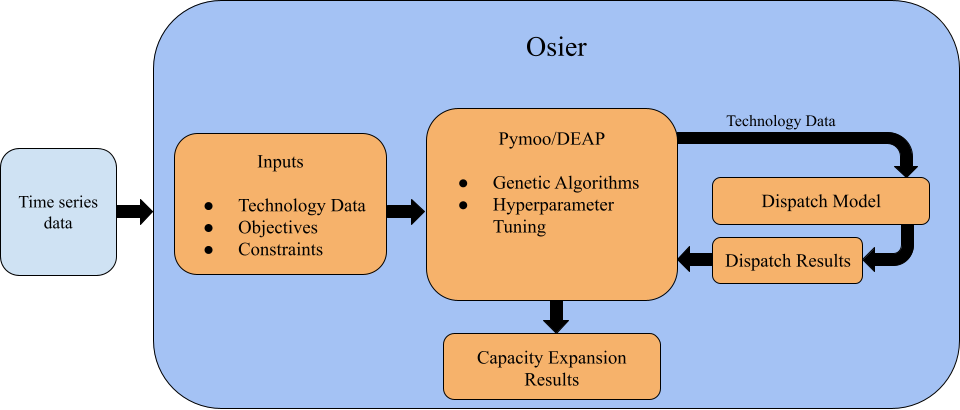
\includegraphics[width=\columnwidth]{figures/osier_flow}
    \caption{The flow of data into and within \ac{osier}}
    \label{fig:osier_flow}
\end{figure}

 Technology data, objectives, constraints, and a dispatch model are all features
within \ac{osier}, while \ac{pymoo} drives the optimization of these objectives.
The dispatch model is independently executable for inspecting specific test
cases and mapping solutions from other solvers onto \ac{osier}'s objective
space. The next section elaborates on the dispatch model's formulation.
